% --------------------------------------------------------------
% This is all preamble stuff that you don't have to worry about.
% Head down to where it says "Start here"
% --------------------------------------------------------------
 
\documentclass[12pt]{article}
 
\usepackage[margin=1in]{geometry} 
\usepackage{amsmath,amsthm,amssymb}
\usepackage[margin=1in]{geometry} 
\usepackage{amsmath,amsthm,amssymb}
%\usepackage[spanish]{babel} 
\usepackage[T1]{fontenc} 
\usepackage[utf8]{inputenc} 
\usepackage{lmodern} 
\usepackage[colorlinks,linkcolor=blue,urlcolor=blue]{hyperref}
\usepackage{graphicx}
\graphicspath{ {images/} }
\usepackage{hyperref} 
\usepackage{indentfirst}
\setlength{\parindent}{2em}
\usepackage{float}
\usepackage[section]{placeins}
\addtolength{\parskip}{0.3em}
 
\newcommand{\N}{\mathbb{N}}
\newcommand{\Z}{\mathbb{Z}}
 
\newenvironment{theorem}[2][Theorem]{\begin{trivlist}
\item[\hskip \labelsep {\bfseries #1}\hskip \labelsep {\bfseries #2.}]}{\end{trivlist}}
\newenvironment{lemma}[2][Lemma]{\begin{trivlist}
\item[\hskip \labelsep {\bfseries #1}\hskip \labelsep {\bfseries #2.}]}{\end{trivlist}}
\newenvironment{exercise}[2][Exercise]{\begin{trivlist}
\item[\hskip \labelsep {\bfseries #1}\hskip \labelsep {\bfseries #2.}]}{\end{trivlist}}
\newenvironment{problem}[2][Problem]{\begin{trivlist}
\item[\hskip \labelsep {\bfseries #1}\hskip \labelsep {\bfseries #2.}]}{\end{trivlist}}
\newenvironment{question}[2][Question]{\begin{trivlist}
\item[\hskip \labelsep {\bfseries #1}\hskip \labelsep {\bfseries #2.}]}{\end{trivlist}}
\newenvironment{corollary}[2][Corollary]{\begin{trivlist}
\item[\hskip \labelsep {\bfseries #1}\hskip \labelsep {\bfseries #2.}]}{\end{trivlist}}

\newenvironment{solution}{\begin{proof}[Solution]}{\end{proof}}
 
\begin{document}
 
% --------------------------------------------------------------
%                         Start here
% --------------------------------------------------------------
 
\title{Group Project Proposal}
\author{Jingying Yin\\ %replace with your name
Yining Zhang}
\maketitle
\section{Team members' responsibility}
\textbf{Jingying Yin}:
	Web visualization design, the script of our website

\textbf{Yining Zhang}:
	Build online database, interaction between website and database
\section{Our data set}
We choose the data set of Google Play Store Apps, which is about the app information on Google Play Store. The reason we selected this is that we care about the mobile market for users. As we all know, people use mobile phones every day for several hours. From this data set we want to figure out which features influence the frequency of app download times and app ranking most.

Our data set has 13 columns, they are App’s name, category, rating, reviews, size, install times, type of purchase, price, content rating, genres, last update time, current version and android version.

Our data set looks like Figure 1.

\begin{figure}[H]
\centering
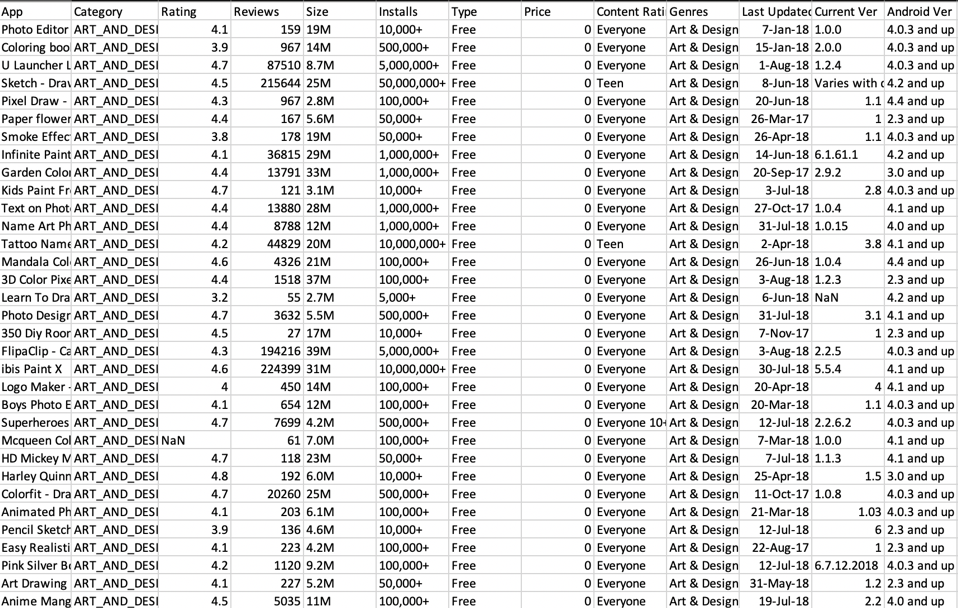
\includegraphics[scale=0.55]{Images/Picture1.png} 
\caption{the overview of data set: Google Play Store Apps}
\label{picture1}
\end{figure}

The link of the data set: \href{https://www.kaggle.com/lava18/google-play-store-apps}{https://www.kaggle.com/lava18/google-play-store-apps} 

\section{Our website designs}
Our website is an online data analyst website. We decide to develop 2 pages to show different attribute.

The First page (Figure 2), the users can view all the data details on the front page as shown below. In this page, the users also can find the description and some simple statistical result of each features. Also, they can sort the data by different features and can use filters to find one or more specific data. On the top of this page there will be a little button, from this users can go to next page.

The second page (Figure 3), this is a more professional page. The user can find some analyze of our data set here, about the distribution of each features, relationship between each 2 features, relevant matrix and they even can draw simple regression among two features. App developers can find advisement for their further development through the consumer behavior from our website.

\begin{figure}[H]
\centering
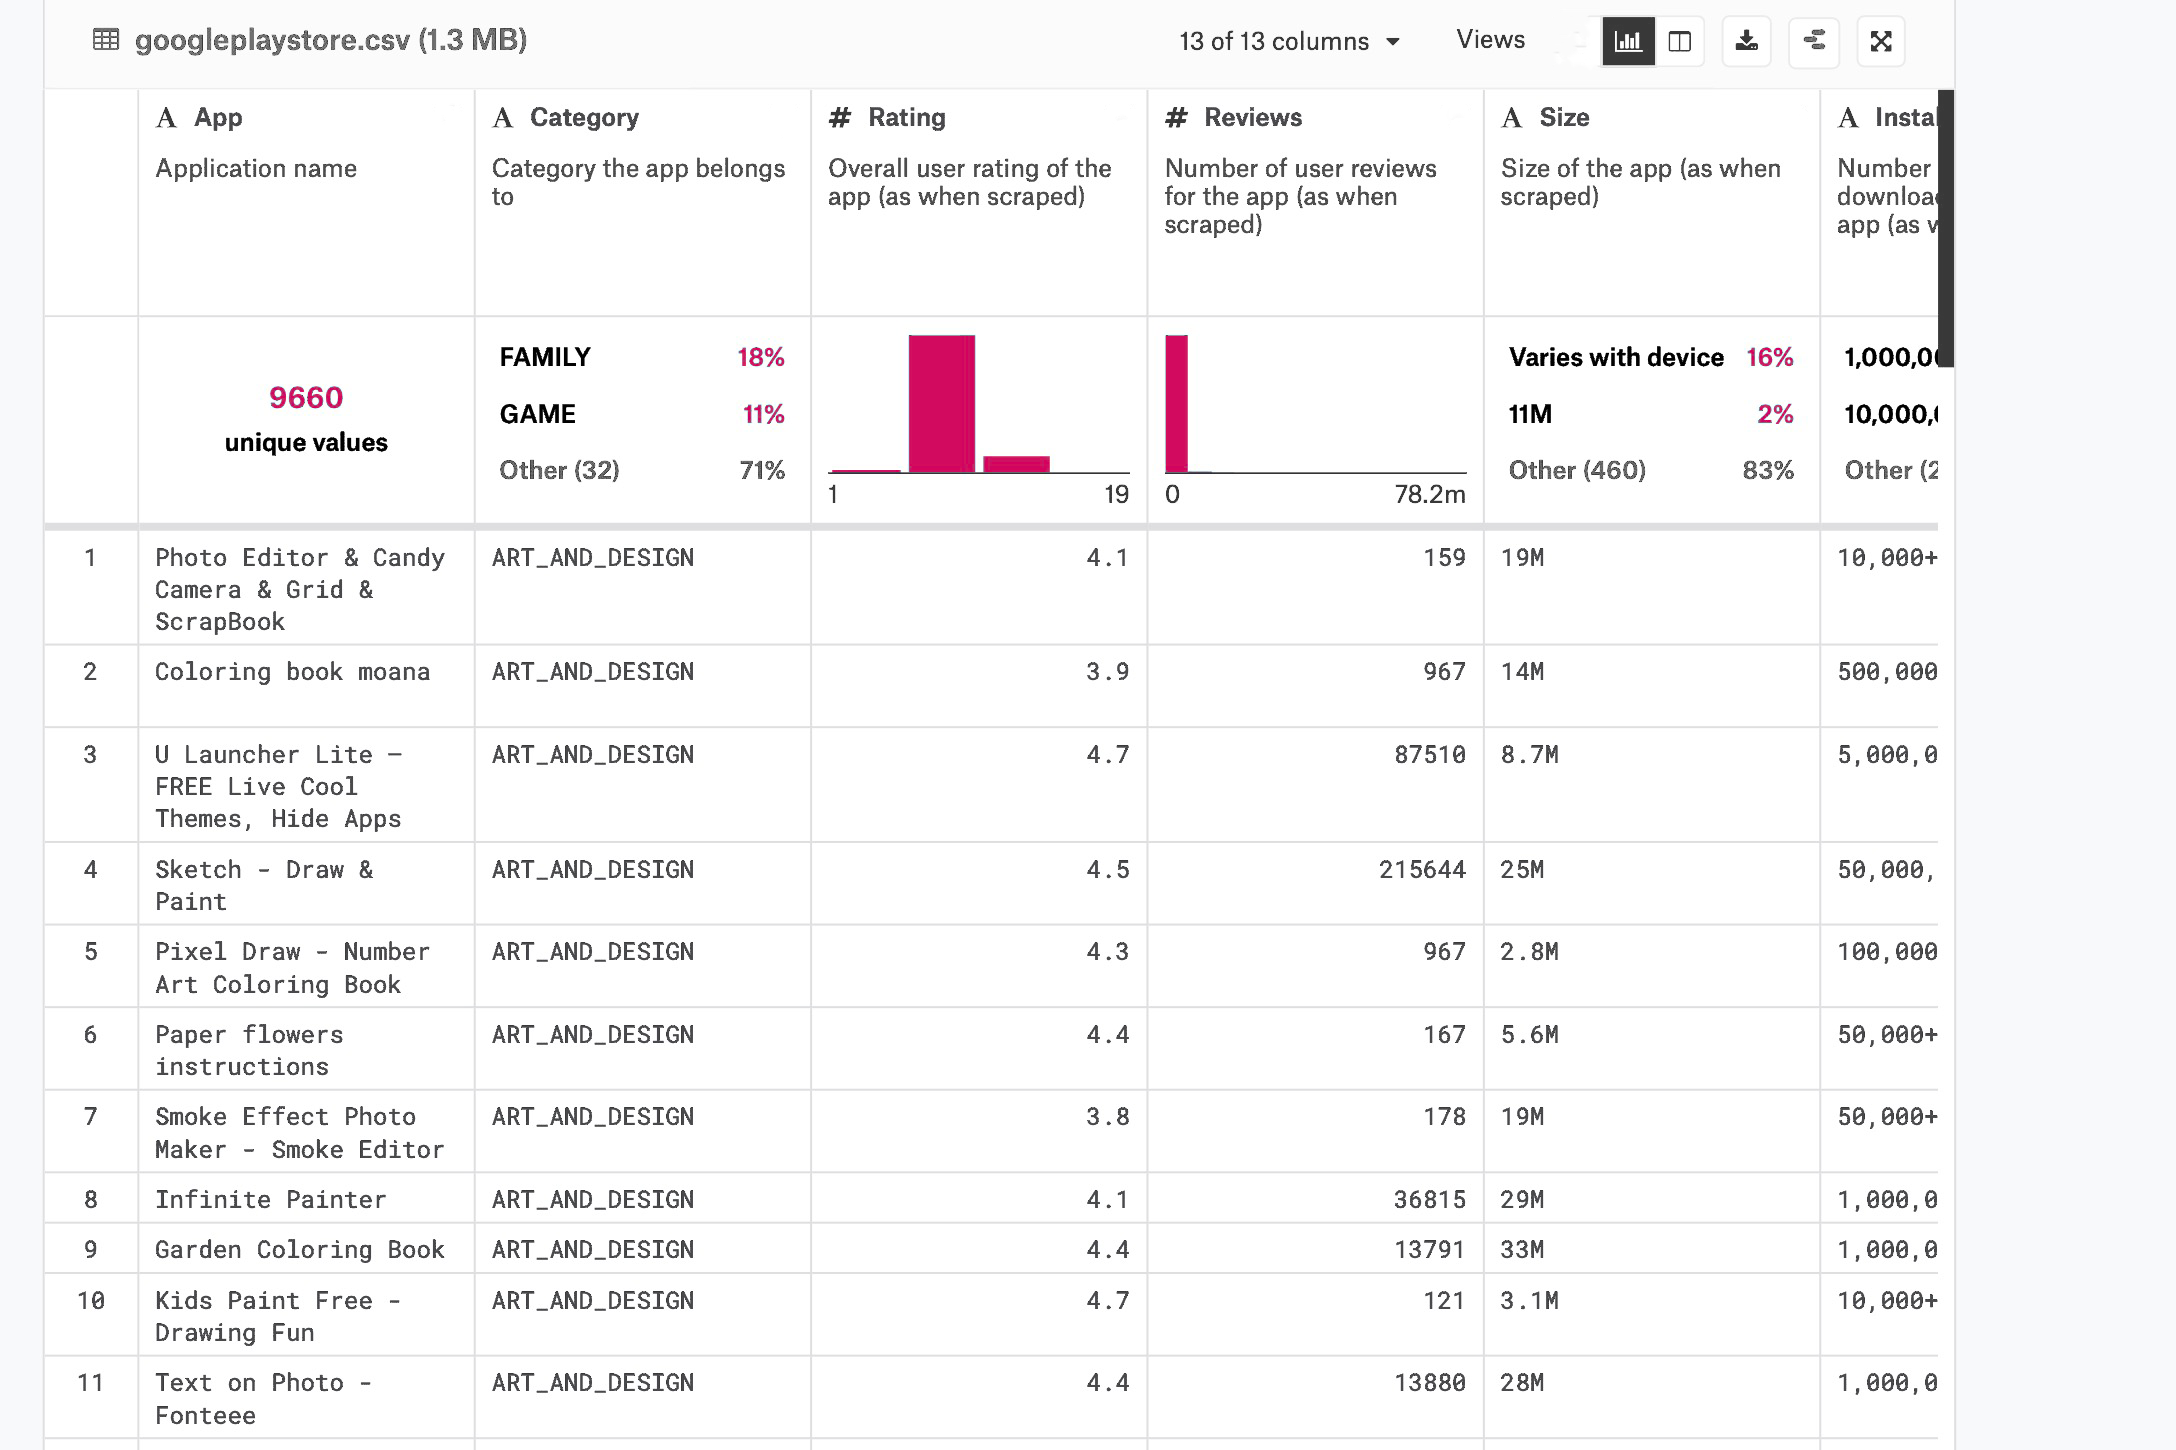
\includegraphics[scale=0.15]{Images/Picture2.png} 
\caption{the front page of our website}
\label{picture2}
\end{figure}

\begin{figure}[H]
\centering
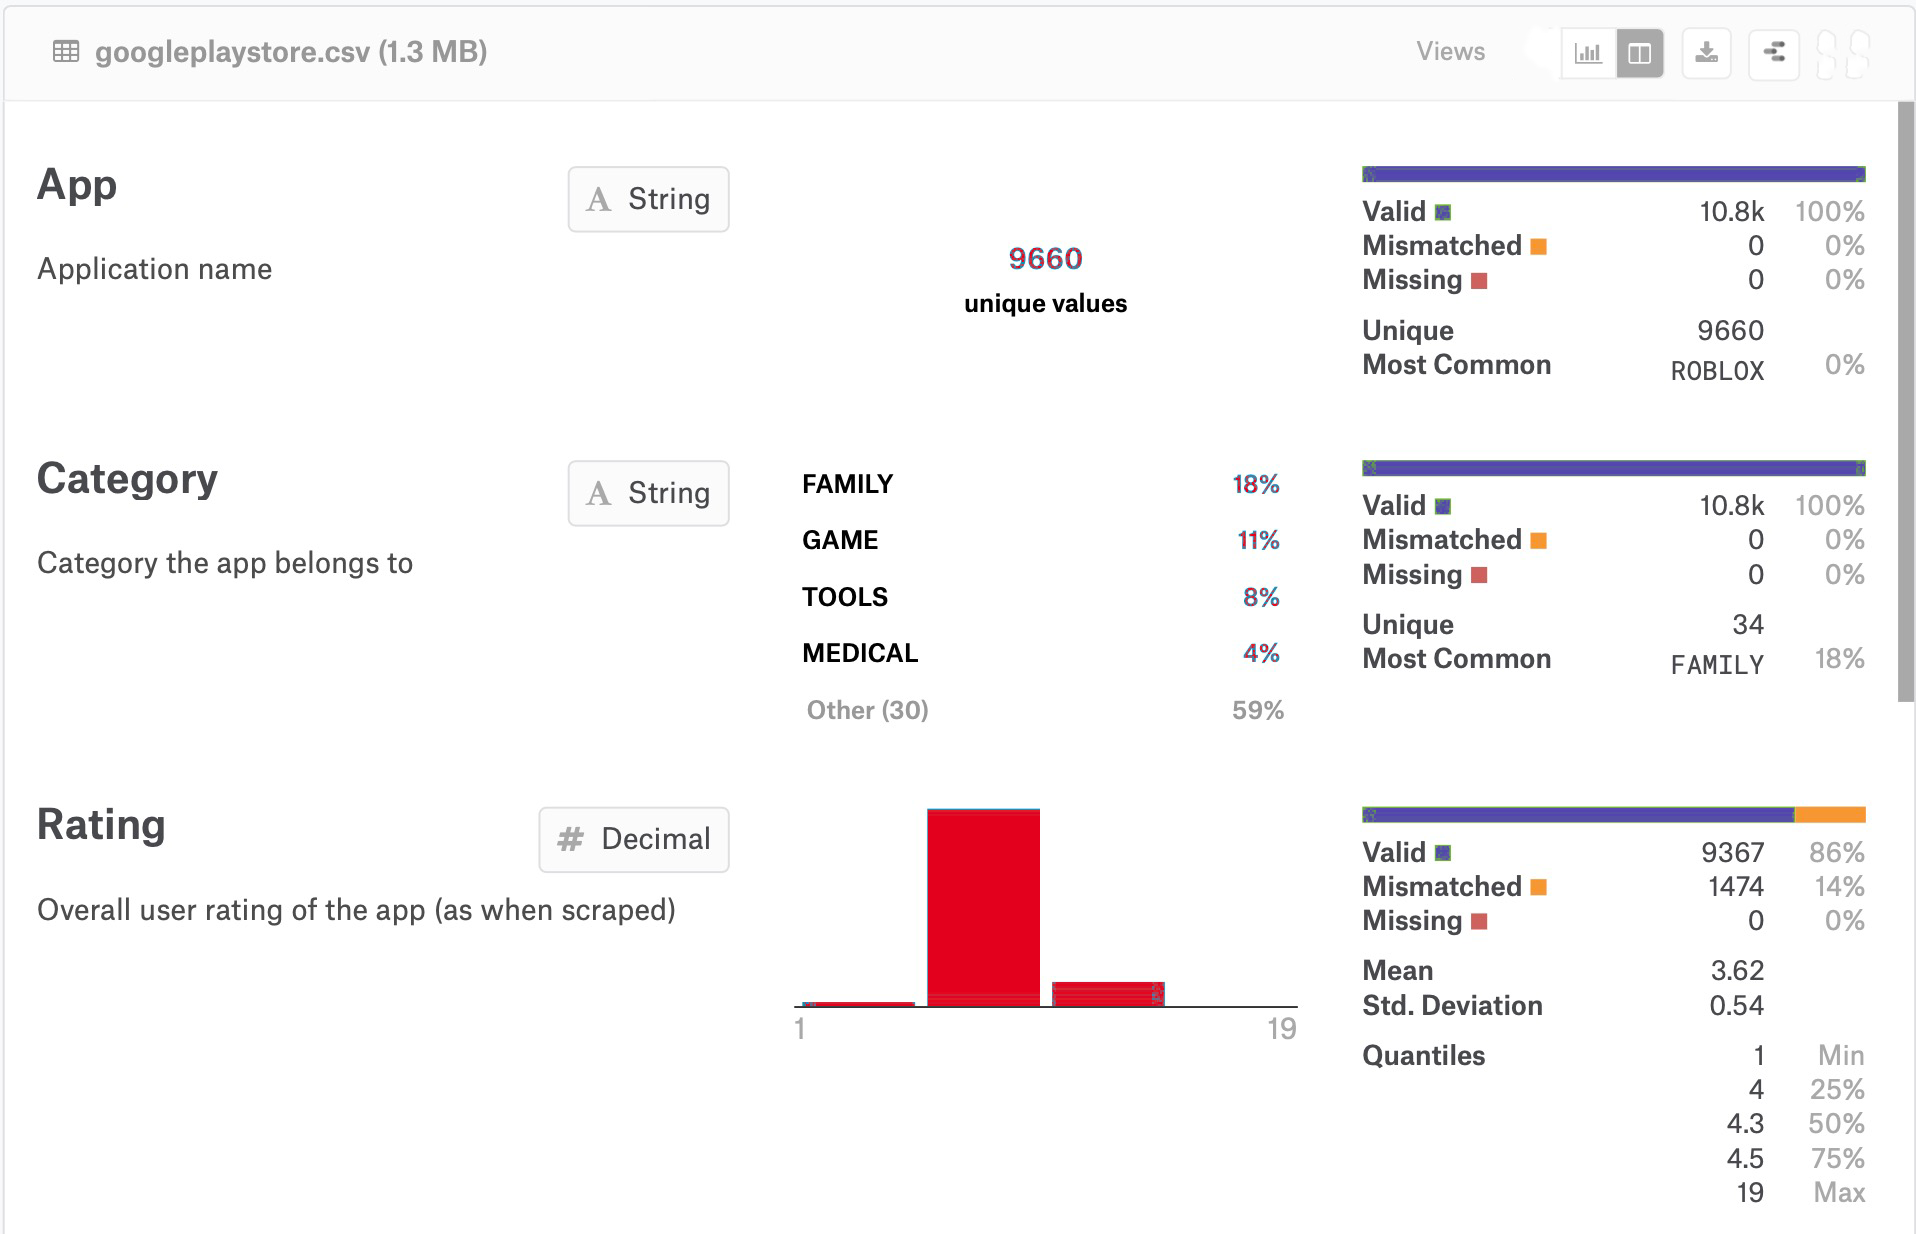
\includegraphics[scale=0.15]{Images/Picture3.png} 
\caption{ the analyst page of the data set}
\label{picture3}
\end{figure}

\section{Programming language}
We use HTML, java script, java to achieve the website UI and the interaction between our website and database.

Also, we choose relational database, such as mySQL as our online database.

\section{Timeline for our project}

\begin{table}[H]
\centering
\caption{Milestone schedule}
\begin{tabular}{{c|c}}   
\hline\hline
 Timeline &tasks  \\  
\hline
9.18,2019 & Finish our proposal\\
\hline
9.28,2019 & Build our online database\\
\hline
10.8,2019 & Website UI\\
\hline
10.18,2019 & Show the data set on the front page\\
\hline
10.28,2019 & Build models for the analysis locally\\
\hline
11.8,2019 & Analyze the data and draw charts and graphs\\
\hline
11.18,2019 & Show the analyze results on the website\\
\hline
11.28,2019 & Show charts and graphs on the website\\
\hline
11.30,2019 & Test all the features of our website\\
\hline
12.2,2019 & Submit our group project\\
\hline

\end{tabular}
\end{table}

\end{document}
